\chapter{Conclusion}

To test the real world performance, we have connected computers to both agents of our system and hosted an Updog (a small program that allows uploading and downloading files via HTTP/S) server on one of them and loaded a page on other computers browser.

\begin{figure}[H]
\begin{center}
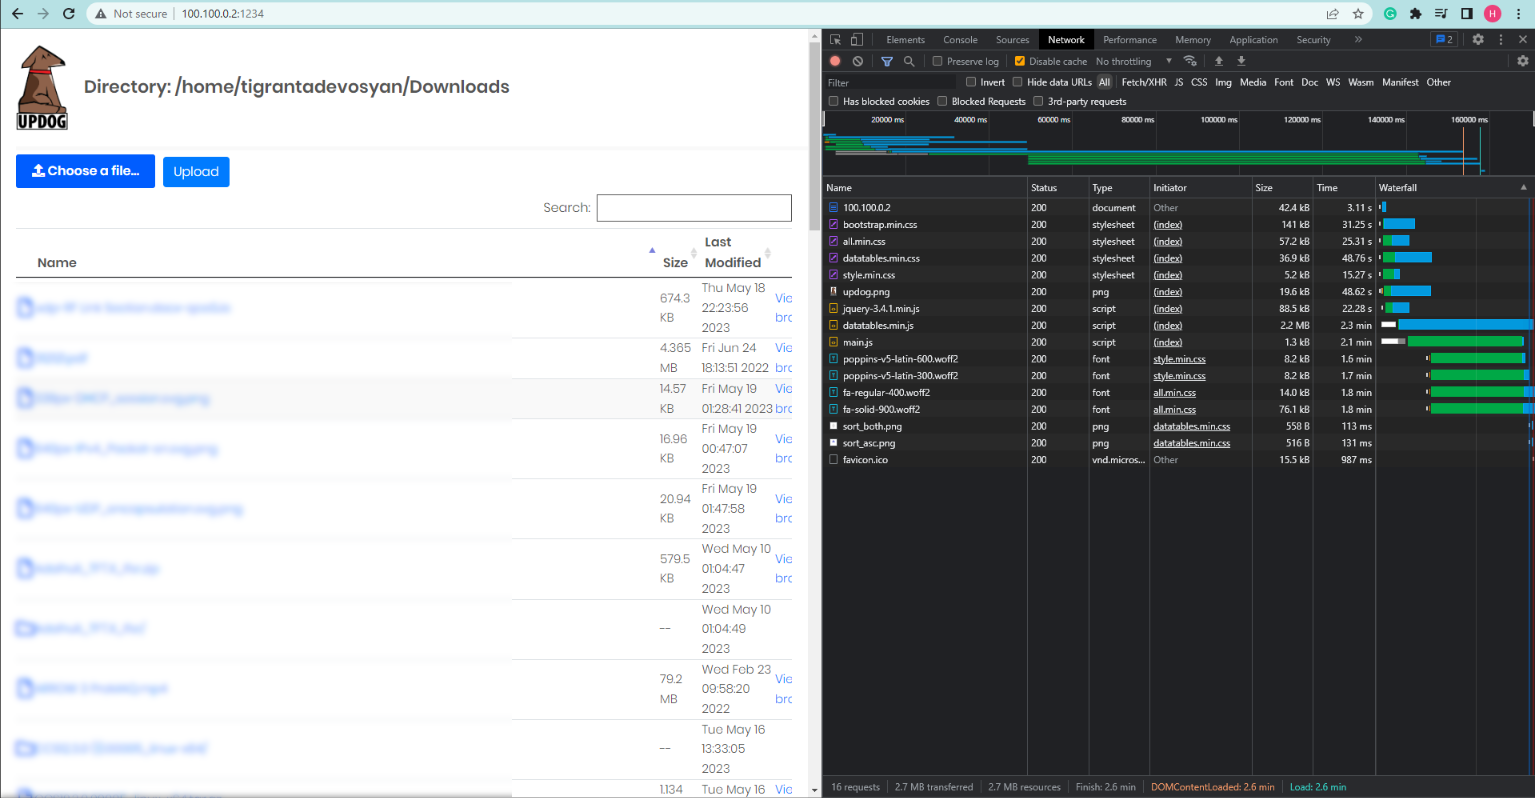
\includegraphics[width=0.90\textwidth]{updog-2.png}
\end{center}
\caption{Screenshot of Updog loaded through our network.}
\label{updog}
\end{figure}

A 2.7 Mb was loaded in 2.6 minutes, which means we had average data speed of 17.3 KB/s. Of course this is not representative of the throughput of the system as 2.7 Mb is just the amount that was finally loaded and there is other traffic going around that is not included 2.7 Mb (for example acknowledgment messages). Moreover, there are going to be some packets that become corrupted during transmission or fragments of the are dropped as the system is overloaded. But in our opinion this metric is more important as it represents the real world capabilities of the system.   

\begin{figure}[H]
\begin{center}
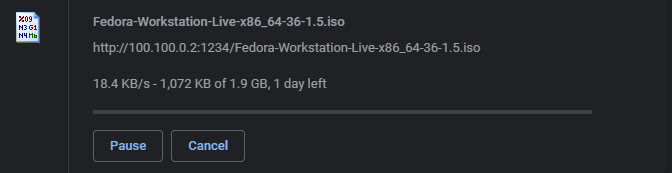
\includegraphics[width=0.90\textwidth]{download.png}
\end{center}
\caption{Screenshot of download a file through our network.}
\label{download}
\end{figure}

Above is a figure of file download process through our system and as it can bee seen, we are able to maintain approximately 18 KB/s of sustained traffic. Of course the is not enough to things that we are accustomed to do through Internet, like streaming an HD video, but it would be more then enough to accommodate file transfer in cases when wired connection is inconvenient or impossible (for example a UAV during flight). Moreover, with the help of modern compression algorithms the throughput is more then enough to facilitate a relatively decent voice streaming. For application where the data rate is low, like text messaging, the system can be used to connect subnetworks with multiple users to each other. 

As it have already been mentioned the main "bottle-neck" for our system's throughput turned out to be the processing power of the RF link. One possible method of increasing it is the optimizing of the source code of the RF link, but the gains that can be achieved this ways are relatively insignificant. A more realistic way would be changing the hardware of the RF link, as a faster MCU would significantly increase the throughput of the system up until other parts of the system become the "bottle-neck". Integration of the system on one circuit would allow us to increase the stability and speed of SPI and UART connections. Moreover, we can increase the Ethernet reception and transmission, by replacing the W5500 with Microchip's first party ETHERNETPHY module.

With the help of Free Space Path Loss equation we have calculated that maximum theoretical distance our radio can work for our maximum output power (+14 dBM) is 12km. Obviously in real world application the maximum range would be closer to 10 km assuming good conditions like relatively low noise in the environment and unobstructed vision. There are three main ways of increasing the maximum operational range: 
\begin{itemize}[nolistsep]
    \item Improving transmission by connecting an external power amplifier,
    \item Using external high gain antennas, 
    \item Improving reception with low noise amplifiers on receiver.
\end{itemize}

Other improvements might be:
\begin{itemize}[nolistsep]
    \item Dynamic assignment of roles and time slots and facilitation of more agents in the network,
    \item Use of multiple antennas to achieve a full-duplex communication or increas overall system throughput in the case of high number of agnets in the network, 
    \item Integration of the system into a complete package, by designing a custom PCB, case, and battery.
\end{itemize}

\begin{figure}[H]
\begin{center}
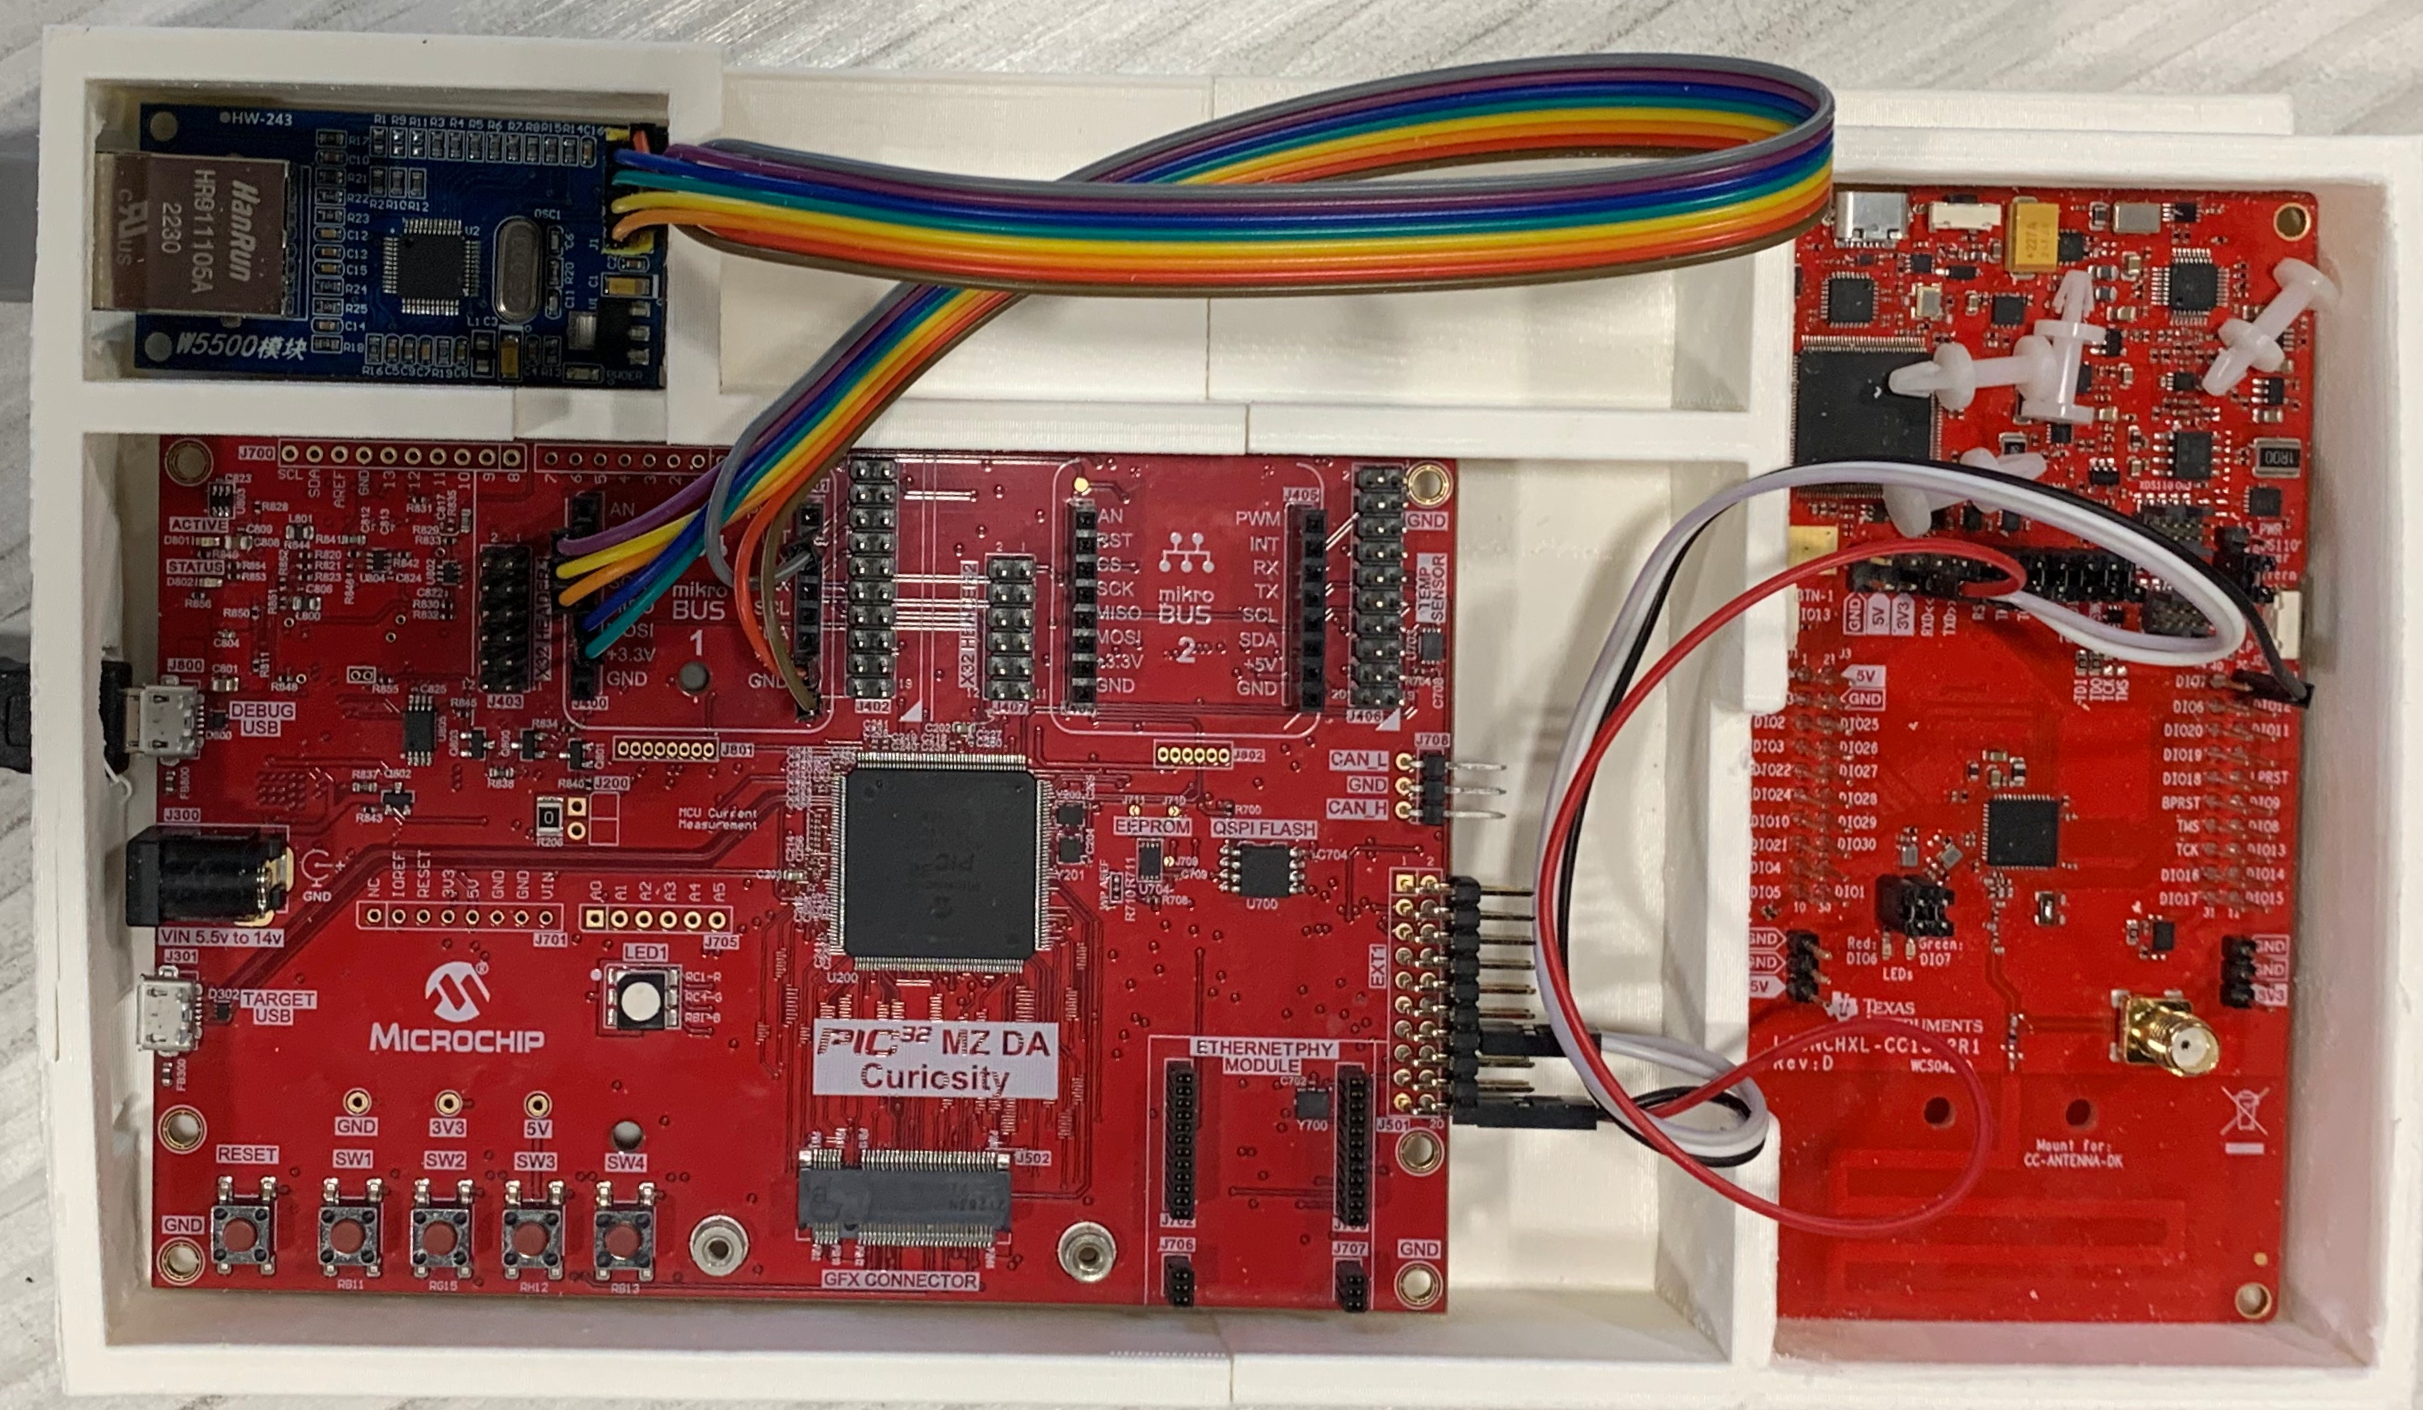
\includegraphics[width=0.90\textwidth]{final.jpg}
\end{center}
\caption{Final result.}
\label{download}
\end{figure}



